%\documentclass{article}
%\documentclass[10pt,twocolumn]{article}
\documentclass[11pt,english]{article}
\usepackage[T1]{fontenc}
\usepackage{babel}
\usepackage[utf8]{inputenc}
%% Sets page size and margins
\usepackage[a4paper,top=3cm,bottom=2cm,left=3cm,right=3cm,marginparwidth=1.75cm]{geometry}

%\documentclass{article}
\usepackage{array}
\usepackage{url}

\newcommand\Mark[1]{\textsuperscript#1}


\date{}

\usepackage{natbib}
\usepackage{graphicx}

\usepackage{multicol}

\begin{document}

\title{Title 01. (Aggressive Action Estimation: A Comprehensive Review on Neural Network Based Human Segmentation and Action Recognition) 
Title 02. (A Comprehensive Review on Neural Network Based Segmentation and Action Recognition) Title 03 (A Comprehensive Review on Vision Based Deep Learning Human Segmentation and Action Recognition)}

\author{\textbf{DR. A. F. M. Saifuddin Saif}\Mark{1}, \textbf{MD Akib Shahriar Khan}\Mark{2}, \\ \textbf{Abir Mohammad Hadi}\Mark{3}, \textbf{Rahul Proshad Karmoker}\Mark{4}, \textbf{Joy Julian Gomes}\Mark{5}\\
\Mark{1} Assistant Professor, Department of Computer Science and Engineering,\\American International University-Bangladesh, Dhaka, Bangladesh\\ \Mark{1}saif@aiub.edu \\
\Mark{2} \Mark{3} \Mark{4} \Mark{5} Student, Department of Computer Science and Engineering,\\American International University-Bangladesh, Dhaka, Bangladesh\\\Mark{2}akeeebkhan@gmail.com, \Mark{3}abir45pro@gmail.com,\\ \Mark{4}karmoker.rahul4@gmail.com, \Mark{5}joyjuliangomes@gmail.com}

\maketitle
\begin{abstract}
Human action recognition has been a talked topic since machine vision was coined. With the advent of neural networks and deep learning methods, various architectures were suggested to address the problems within a context. Convolutional neural network is been the primary go-to architecture for image segmentation, flow estimation and action recognition in recent days. As the problem itself is a extended versions of various subproblems, such as frame segmentation, spatial and temporal feature extraction, motion modeling and action classification as a whole, some methods reviewed in this paper addressed subproblems and some tried to address a single architecture to the action recognition problem. While being a success, convolution neural network have drawbacks in its pooling methods. CapsNet, on the other hand, uses squashing function to determine the activation. Also it addresses spatiotemporal information with the normalized vector maps while CNN-based methods extracts feature map for spatial and temporal information and later augment them in a fusion layer for  combining two separate feature maps. Critical review of papers provided in this work can contribute significantly in addressing human action recognition problem as a whole.
\end{abstract}

\section{Introduction}
Action recognition in videos can have a radical impact on human life. Numerous attempts has been taken to solve the action recognition challenges. Due to huge collaborative efforts in computer vision community, simple actions of waving, standing etc. from KTH and Weizmann dataset are now considered as obsolete challenges and the community has moved on to solve more complex actions like sports and human interactions. However, despite having the potential to improve security and surveillance applications, there has not been much improvement in regard to the violent scene and aggressive behavior, which is a special case of action recognition.

Previous works on action recognition heavily relied on usage of hard coded techniques such as MoSIFT, Optical Flow and Dense Trajectory. These hard coded techniques are computationally expensive while offering low performance. In recent times after the success of AlexNet a wave of  works approached the problem from a new viewpoint using convolutional neural networks. Though being incisive in image classification tasks, Convolutional Neural Networks did not fare well with already established methods immediately. Different types of fusion techniques using both dense features and CNN improves performance. 2-stream networks and 3D-CNN using motion features such as optical flow and RNN in conjunction of afford mention techniques also gave a boost in performance. But these approaches have some severe disadvantages like max-pooling which in most cases suppresses tiny but important features and, susceptible to adversarial attacks. Though these methods work, they do not provide any insight on how the inner mechanism functions. The newly proposed CapsNet architecture can help to bridge the gap as this particular system follows a part-to-whole approach and produces vector outputs unlike CNN which has scalar outputs. Capsules are particularly good at handling different types of visual stimulus and segmenting pose(position, size, orientation),  deformation, velocity, albedo, hue, texture etc. which is not possible for CNN.Capsules encapsulate all-important information about the state of the feature they are detecting in vector form.


The rest of the paper is organized as follows. Section 2 discusses challenges of action recognition and provides a concise view on broad range of technologies and approaches that are used to solve the problem. In section 3 numerous methods related to action recognition are reviewed. Section 4 elaborates the frameworks used in the method described in section 3. Section 5 provides details on the experimental settings and performance of the methods. In section 6 key findings from the methods are summarized. In section 6.1 a new framework is proposed. Section 7 concludes the paper emphasizing the impact of the problem. 



\section{Core Background Study}
Human action recognition is an integral problem in spatiotemporal information extraction, fusion, learning and detection from video streams, both in static and especially in a live feed analysis. Numerous studies have been conducted based on hard-coded feature extraction, pose estimation, frame and dynamics and also as neural network learning problem. The problem in discussion is addressed by sub-problems that include: frame preprocessing (if any), feature extraction (both spatial and temporal), learning the feature sets and classification. Further dividing the problems of feature extraction includes background subtraction for subject(s) isolation and background dynamics for temporal information gathering. For learning the problem is subdivided into two categories: individual action and social action where the individual's actions are considered as collective action within the context.

 \begin{figure}
\centering
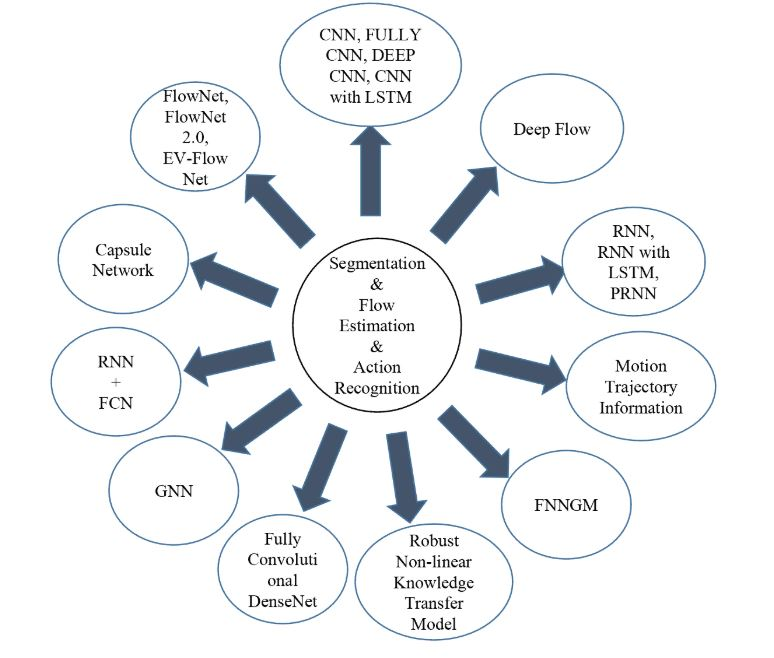
\includegraphics[width=0.7\textwidth]{methods.JPG}
\caption{\label{fig:method}Existing methods for segmentations and action recognition.}
\end{figure}

Feature extraction is addressed by single-frame detection for the subject identification (E.g.: Human) and multi-frame detection for the flow field estimation that gives subjects’ collective movement modeling. \citep{datta2002person} Addressed the collective problem with hard-coded feature extractor for probabilistic model generation which used adaptive background subtraction for human silhouette segmentation and color sum square difference for motion modeling. They used Acceleration Measure Vector and jerk modeling which classifies action as violent or not. \citep{bagautdinov2017social} Addressed the individual person action recognition problem by dense feature representation to obtain feature maps and further refining by inference in a hybrid Markov Random Field. Feature maps are then passed through RNN layer to analyze according to temporal domain. \citep{xiao2017human} Uses autoencoder to train for both human body segmentation and motion modeling. Then a deep network is used to perform action recognition. \citep{zhu2018ev} Also uses encoder-decoder networks to address the problems. In \citep{jegou2017one}, dense feature maps are also used and fully convolutional DenseNet is used to get the output. \citep{baccouche2011sequential} Used 3D-CNN to train the feature and motion model and RNN with LSTM are used to perform action recognition. \citep{sun2017lattice} Also used CNN for two-stream network which independently calculates spatial and temporal features. Then applies recurrent attention mask to regularize and the modified RNN produces more complex and intricate motion features. \citep{chen2017semi} Addresses action recognition in extremely low resolution videos using a semi-coupled ConvNets which share some common filters and some stream-only filters to train and test the data. \citep{dosovitskiy2015flownet} and \citep{ilg2017flownet} presents optical flow estimation as a learning problem and uses ConvNets to predict the optical flow. \citep{ilg2017flownet} further extends the problem to data scheduling showing an interesting insight that scheduling training data improves the performance on most of their tested datasets.  \citep{pigou2018beyond} Addresses spatial and temporal information extraction and learning using a strategic temporal pooling using ConvNets with average pooling and bidirectional RNN sequence. \citep{luvizon20182d} uses stacking of 2D pose probability heat maps to generate 3D pose estimation and uses Fully Connected Networks to aggregate the pose-based and appearance-based action estimations. \citep{oyedotun2017deep} uses multilayer CNN and Stock Denoising Autoencoder layers for training and testing. In \citep{wang2017spatiotemporal}, authors tried to mitigate the misclassification arised using two-stream networks where they used Spatiotemporal Compact Bilinear Fusion (STCB) that can back-up spatial stream with temporal stream and vice versa. \citep{rahmani2018learning}, \citep{zhang2017view}, \citep{zhang2017geometric}, \citep{li2017end} and \citep{li2018action} uses skeleton information to train their system. \citep{rahmani2018learning} uses dense trajectory calculation and encoding the shape of the trajectory for training and learns through knowledge transfer model while \citep{zhang2017view} and \citep{zhang2017geometric} utilizes LSTM to extract and learn temporal dynamics. \citep{yue2015beyond} uses stacked LSTM layer with SoftMax for prediction. \citep{sabour2017dynamic} Uses a completely different approach than all other literature mentioned above. 
Recent development in feature detection and extraction has seen a massive leap ahead with the invention of CapsNet\citep{sabour2017dynamic}. This method allows tiny features to be detected in low level and provides vector data rather than a scalar. The vector data holds key to improve optical flow estimation. With orientation and magnitude of feature data being embedded in the capsule output, it is possible to calculate the difference in orientation and magnitude between two frames with positional transitions.


\section{Review Based on Methods}
Capsule network architecture \citep{sabour2017dynamic} recognise overlapping digits by segmentation and reconstruction. Here, CapsNet layer is a nested layers of convolutional layers which outputs activation vectors. Later by using the vectors the reconstruction process is completed. The capsule network algorithm starts with the primary convolutional layer. The primary convolutional layer consists of 256, 9x9 kernels and a ReLU activation. This Convolutional layer converts pixel congestions to the activity of local feature detectors which are used as input to the primary capsules. In Capsule layer Capsules encapsulate all important information about the state of the feature they are detecting in vector form. These Capsules encode probability of detection of a feature as the length of their output vector as well as the state of the detected feature is encoded as the direction in which that vector points to. Instead of scalars, the neuron level is stored as vectors. These vectors contain information about: 1. spatial orientation, 2. magnitude/prevalence, and 3. other attributes of the extracted feature.
Segmenting regions \citep{lalonde2018capsules} used Capsule network with an added SegCaps layer and \citep{afshar2018brain} decreased the feature map count from the main Capsule Network architecture. A descriptor matching algorithm \citep{weinzaepfel2013deepflow} which allows to boost performance on fast motions. It allows to efficiently retrieve quasi-dense correspondences and handle large displacements. Since capsnet can handle small number of training samples, and units in these networks are equivariant, they outperform CNN.
Estimating the optical flow FlownetS \citep{dosovitskiy2015flownet} consisted generic CNN allowing the network to decide itself the processing of a pair of the images. FlowNetC\citep{dosovitskiy2015flownet}  is constructed such a way, it takes 2 different input at a same time to produce a meaningful representations of the two images separately and then standard matching approach is followed. FlowNet 2.0 \citep{ilg2017flownet} is constructed by stacking FlownetS and FlowNetC. Two separate streams were introduced with one responsible for detecting large displacement and another for small displacement and the fusion happens in the later stage. The precision on this model is four times higher than with the first FlowNet.
 FlowNet2.0 has higher accuracy for having a large model by using stacked structure and fusion network. As for stacked structure, Flownet2.0 estimates large motion in a coarse to fine approach, by warping the second image at each level with the intermediate optical flow, and compute the flow update. The EV-FlowNet\citep{zhu2018ev} architecture very closely resembles the encoder-decoder networks. This method learns optical flow using events as inputs only, without any supervision from ground-truth flow.
To recognize action recognition at extremely low resolution a fusion technique of two-stream networks\citep{chen2017semi} with a spatial ConvNet and a temporal ConvNet is used. Later a fully connected layer provides the output. Regression based deep CNN\citep{luvizon20182d} method is used to extend ta 2D pose to 3D pose estimation by stacking the heat maps. Finally a fully connected network extracts the pose features using max-pooling and softmax activation. In \citep{wang2017spatiotemporal} Spatiotemporal Compact Bilinear Fusion (STCB) method is used to counter misclassification in two-stream spatiotemporal network by introducing a way of bilinearly fusing spatial and temporal information using a modified LSTM-RNN network. In \citep{oyedotun2017deep} showed a method of Multiple variation of hidden layers are trained in different CNN layers and total neuron counts vary in different layers of SDAEs to recognise different hand gestures. \citep{yue2015beyond} works expending temporal length in video descriptor as descriptor with longer temporal range are more robust and discriminative.This paper also evaluates different approach to feature pooling. Temporal Segment Network \citep{wang2016temporal} is a 2 stream network aims to model long range temporal structure modeling. It employs a sparse temporal sampling strategy to effective learning. \citep{wu2015modeling} proposes a hybrid deep learning framework for video classification and able to model static spatial information, short-term motion, as well as long-term temporal clues in the videos. In paper \citep{sun2017lattice} a preprocessing operation is followed by  passing video flow through CNN stream for spatial information extractor and CNN stream for temporal information extractor. Later Lattice-LSTM learns independent memory cell transition through the shared control gates. \citep{shi2017sequential} proposes a long term motion descriptor to capture spatial, short-term motion and long-term motion features. To achieve this dense trajectory is projected onto 2 dimensional feature space and this feature map is used in a CNN-RNN networks to extract spatial and motion features. Paper \citep{baccouche2011sequential} showed an architecture combined with  2 alternating convolutional, rectification and subsampling layers which is later joined by a final convolutional layer. Standard Backpropagation with momentum algorithm, adapted to weight sharing. used to train the architecture.  In order to classify the action sequences, a Recurrent Neural Network architecture with one hidden layer of LSTM cells is used. \citep{he2016deep} Proposes Region Proposal network, an algorithmic change in previous image segmentation works (RCNN, Fast-RCNN) which leads to dramatic speedup in image segmentation with nearly zero computation for candidate bounding box proposal. While another method \citep{bagautdinov2017social} used dense feature representation for every frame. Here feature maps are then passed to a matching RNN that analyze according to temporal domain. Output of this are the probabilities of an individual's action and the collective activity over time.
 A cluster of temporal convolution and recurrence \citep{pigou2018beyond} is used to determine gestures where CNN remains same as single-frame baseline model but on above that a bidirectional RNN is implemented to compute two hidden sequences, forward hidden sequence and backward hidden sequence. The RNN layer uses LSTM cell because LSTM cells retain their memories much longer than standard cells. Finally a softmax classifier used at the end to predict the result.
 

 
Fully Convolutional Network and DensNet methods are composed and results in Fully Convolutional DensNet\citep{jegou2017one} known as Tiramisu Neural Network. FCNs are created by downsampling path, upsampling path and skip connections. Later they were combined and created the main architecture to determine actions. Paper\citep{xiao2017action} used fuzzy neural network and graph model construction method to recognise actions. Here Fuzzy C Mean is used to obtain representative frames and later FNN classifies them. This method has great Frame accuracy and video accuracy even higher than SVM, NN, CRF, NNCRF methods. 
In \citep{li2017end} skeleton joints are transformed into unified joint coordinates and fed into a deep convolutional network. Later the generated images are fed into a pretrained VGG-19  model to perform fine-tuning and action recognition. Paper \citep{zhang2017view} explores into action recognition through 3D skeletal video temporal and spatial information. For the spatial information, the method detects the global coordinate of the skeleton with respect to camera sensor, then dynamically adjust the position through adaptive LSTM by creating a new virtual camera viewpoint. Geometric Features for Skeleton-Based methode \citep{zhang2017geometric} is used to classify action sequence. Here LSTM architecture are stacked with 3 layers. Bottom layer is the input layer and 3rd layer outputs to SoftMax layer for classification. 
Using Graphical Neural Network \citep{li2018action} showed another weighting approach to adaptively recognize striking activity units for various human activities, which advances human activity acknowledgment precision as well as favors our subjective comprehension to human activities. 
Proposed method has a new weighting way to adaptively detect salient action units for different human actions, which not only promotes human action recognition accuracy but also favors our cognitive understanding to human actions. Paper \citep{edwards2016graph} explored the use of graph based signal-processing techniques for convolutional networks on irregular domain problems.The authors evaluated two methods of graph pooling operators and report the effects of using interpolation in the spectral domain for identifying localized filters. 
\citep{zhang2018semi} Propose a novel semi-supervised learning framework for violence detection, which is suitable for very large data sets. The dictionary is learned from labeled samples for discrimination as well as a large number of unlabeled samples and learning from unlabeled data further increases its representative power. \citep{szegedy2015going} Proposes a dictionary learning based novel method for violence detection, which is suitable for very large data sets. The dictionary is learned from labeled samples for discrimination as well as a large number of unlabeled samples and learning from unlabeled data further increases its representative power; In ref. \citep{datta2002person}, \citep{nievas2011violence} motion trajectory and bag of words analysis are used for violence action detection. Robust Non-linear Knowledge Transfer Model \citep{rahmani2018learning} is used to transfer feature knowledge gathered from dense trajectory for optical flow.
A cascade \citep{weinzaepfel2013deepflow} of DispFluNet and DispResNet is used to determine the stereo matching. An Autoencoding\citep{xiao2017human} method with pattern recognition neural network is used to segment human body and recognise certain actions.
 

\section{FrameWorks}
CapsNet \citep{sabour2017dynamic} architecture has two distinct part. The first first is the encoder which is responsible for delivering a vector for class labeling. The second part is decoder which can recreate the original input based on the output of encoder. Capsnet inspired frameworks tweaks the architecture by varying the input dimensions and number of output channels in the convolution layer. When the detected feature moves around the image or its state somehow changes, the probability still stays the same as length of vector does not change, but its orientation changes. Among the nested capsule layers the length of the output vector of a capsule is assumed to represent the probability that the entity represented by the capsule is present in the current input. A non-linear "squashing" function used to shrunk the short vectors to almost zero length and long vectors get shrunk to a length slightly below 1. The squashing function gets applied to the vector output of each capsule.

The length of all activity vectors extracted from the capsule layer are stored in Vector Caps which indicates the presence of an instance. The CapsNet will detect individual feature present in the frame and extract activation vector. From there it is possible to obtain the specific feature vector orientation and magnitude. In \citep{afshar2018brain} Inputs to the model are MRI images, in order to reduce the number of parameters in the model and decrease the training time. Second layer is a convolutional layer with filters and stride of 1. The second layer is a Primary Capsule layer resulting from convolutions with strides of 2. This layer consists of  “Component Capsules” with dimension. Final capsule layer includes 3 capsules, referred to as  “Class Capsules,’ ’one for each type of candidate brain tumor. CapsNet for object segmentation \citep{lalonde2018capsules} a image is provided as input to the Convolutional layer with a kernel. Later the output is fed into nested Primary Caps layer. SegCaps layer receive output and combined the segmentation. Then fully connected Reconstruction Layer reconstruct the image and provides Output of Segmented Images then masked reconstruct of Positive input class.
2 images are stacked\citep{dosovitskiy2015flownet} in the input and fed through a generic CNN allowing the network to decide itself the processing of the pair of the images to extract the motion information. \citep{ilg2017flownet} describes a way to estimate optical flow using CNN. This framework makes use of FlownetC and FlownetS  is, a generic CNN which is fed two stacked frame and let itself determine the relation between input-output using sliding window  and extract motion information.EV-flownet proposed in \citep{zhu2018ev} is an event-based camera which track the changes in the log intensity of an image, and returns an event whenever the log intensity changes over a set threshold.



For predicting  per pixel flow only the event timestamp images are pass \citep{chen2017semi} Fusion of two-stream networks, a spatial ConvNet and a temporal ConvNet. Fusion function f:f(xs, xt) -> yn where xs is nth spatial layer output and xt is nth temporal layer output. The optical flow of the interpolated eLR frame is calculated. \citep{luvizon20182d} train network using elastic net loss function to predict pose and localize ground truth region with bounding box. If a body joint falls outside the bounding box the ground truth flag is set to 0  else 1. This GT information is used to supervise the joint visibility vector prediction with binary cross entropy loss. In case of action recognition it trained by using categorical entropy loss. In \citep{wang2017spatiotemporal}, To counter the misclassification in two-stream spatiotemporal network by introducing a way of bilinearly fusing spatial and temporal information. For this they coined a method Spatiotemporal Compact Bilinear Fusion (STCB). For explicitly computing outer product without increasing dimensional parameters multiplicatively, the authors used Convolutional Count Sketch method. For temporal fusion they used previously mentioned STCB method. They deploy a Spatiotemporal Attention which is implemented in the last convolutional layers. This module reduces feature map to a feature vector. After that two convolutional layers, sizing are stacked to generate the attention weights for the feature maps. Lastly, the output is normalized using SoftMax layer and combined with the original spatial features by a weighted average pooling layer.In \citep{oyedotun2017deep}, Preprocessing original grayscale images into binary representation for segmentation. The black and white (binary) images are obtained by thresholding the grayscale image levels at 0.5. Binary images are then further filtered using a filter for denoising. Then Stack Denoising Autoencoders (SDAEs) are trained with varying depths to determine any observable improvements. In \citep{yue2015beyond},  Multiple pooling techniques were discussed. In conv pooling the model performs max pooling over the final convolutional layer across the video’s frames. The late pooling pools features after the activations go through the fully connected layers. Slow Pooling performs max pooling is first applied over frames of convolutional features with stride 5. Each max-pooling layer is then followed by a fully-connected layer with shared weights. Another pooling layer works on all the outputs of last fully connected layer. In local pooling pool operation directly performed on last convolution output. Time domain convolution focuses on capturing local relation among frames with 256 filters of 3 x 3 kernels and max pooling is performed on temporal domain. In \citep{pang2017cascade}, The matching algorithm builds upon a multi-stage architecture with 6 layers, interleaving convolutions and max-pooling, a construction akin to deep convolutional nets. Using dense sampling, it allows to efficiently retrieve quasi-dense correspondences, and enjoys a built-in smoothing effect on descriptors matches, a valuable asset for integration into an energy minimization framework for optical flow estimation. Two Segment Network \citep{wang2016temporal} Temporal CNN uniformly and sparsely samples short snippets of temporal data over long period breaking the video data into multiple segments. Segments are later aggregated and consensus among them is the video level prediction. \citep{wu2015modeling} In this framework spatial feature extraction is done with a spatial CNN. Motion CNN extracts motion feature from the stacked optical flow. Regularized feature fusion extracts from spatial and motion CNN and they are fused to make predictions. In \citep{sun2017lattice}, For preprocessing, video clips and their flow field is passed through CNN stream for spatial information extractor and CNN stream for temporal information extractor. Both the image and flow field are fed simultaneously. Here Lattice-LSTM learns independent memory cell transition through the shared control gates.The learned recurrent attention mask further regularize, the output gate produces more complex and intricate motion features. In \citep{baccouche2011sequential}, Two neuron layers contain a classical multilayer perceptron with one neuron per action in the output layer. standard online Backpropagation with momentum algorithm. In order to classify the action sequences, Recurrent Neural Network architecture with one hidden layer of LSTM cells. \citep{shi2017sequential} is a 3 stream network, divided into spatial and temporal part. Temporal part consists of short term and long term subsystem. A simplified version of dense trajectories is first extracted from multiple consecutive frames to represent the motion from body movement or the relative motion between the camera and objects. Then a set of trajectories are projected onto a canvas, consequently resulting in a trajectory texture image. Based on these images, a CNN can be employed to learn a macroscopic representation of motion. To model the dependence on the temporal domain, we consider each Trajectory Texture image as a unit and try to model them in the temporal domain with the LSTMs network.
In \citep{he2016deep},  Deep CNN layers take raw image input and outputs convolution feature volume Region Proposal Network (RPN) and detection network. RPN outputs rectangular object proposals with objectness score. These proposal boxes are used in Fast RCNN Detector. At each sliding point anchor reference boxes are projected. This maps to a grid like structure for the previous feature map. RPN projects anchor which is reference box in different scale and shape to Bounding Box Regression and Objectness Score predictor.  In \citep{bagautdinov2017social}, the method allows to extract features individually for each object which is useful when reasoning about collective behaviors. To achieve the goal dense feature representation is shared between the detection and action recognition tasks. Those detections are refined jointly by inference in a hybrid Markov Random Field (MRF). Resulting bounding boxes are then used to smoothly extract fixed-size representations and used as input of RNN to evaluate probabilities of individual actions for each detection, along with the probabilities of collective activity. In \citep{pigou2018beyond}, Deploying bidirectional RNN is a way to create a "temporary buffer" or "internal memory". The CNN remains same as single-frame baseline model but on top of that a bidirectional RNN with LSTM is implemented to compute two hidden sequences, forward hidden sequence and backward hidden sequence.  In \citep{szegedy2015going}, Consists of repeating blocks of inception module followed by a common convolution and pooling layer. Each inception module is built with 4 towers pooling layer. All of them use ReLU activation. At the end of convolution operations, feature maps are concatenated in a single output vector.  In \citep{jegou2017one}, Fully Convolutional Network and DensNet methods are composed ans results in Fully Convolutional DensNet FCNs are built from a downsampling path, an upsampling path and skip connections. In \citep{xiao2017action} first the frame features of actions in a motion dataset are extracted automatically and cluster frames using the Fuzzy C-Mean (FCM) to obtain Representative Frame (RF)s. Identify RFs gestures using FNN classifier then classify the RF sequence by using a probability graph model named FNNGM. On action recognition section, The unknown action RFs are extracted automatically then obtain action semantic classification results using the FNNGM inference algorithm. 
Paper \citep{li2017end} proposes a CNN method which distinguishes human action based on skeleton joints: hip center, right and left shoulder. Data preprocessing is done to normalize and filter the skeleton joints as unified coordinate system.
In \citep{zhang2017view}, This paper explores into action recognition through 3D skeletal video temporal and spatial information. The method detects the global coordinate of the skeleton with respect to camera sensor, then dynamically adjust the position through adaptive LSTM by creating a new virtual camera viewpoint. The main LSTM network is designed with stacking 3 LSTM network sequentially and a fully connected layer at the end with a SoftMax classifier. The whole system allows to retain temporal dynamics information for longer period and end-to-end training feasible. In \citep{zhang2017geometric}, An stacked LSTM architecture with skeleton temporal information learning to counter the overfitting problem with the frameworks without domain knowledge. The method includes geometric representation of skeleton joints to devise a relation between actions. properly hand crafted features can be valuable to deep learning at it imposes a more natural way of representing the learning problem. LSTM architecture are stacked with 3 layers. Bottom layer is the input layer and 3rd layer outputs to SoftMax layer for classification. To match with the LSTM learning method which is variation over time, they encode 8 types of geometric feature in a single pose.
In \citep{li2018action}, The input is a movement grouping of skeletons, in which each skeletal joint is depicted as a 3D arrange (x; y; z). For each skeleton at one time slice was modeled into an undirected attribute graph, where each skeletal joint is one node and the bone between two joints is considered as one connected edge. Gaussian kernel method is used to weight the graph edges Connected =1 disconnected =0. An action-attending layer is integrated to detect salient action units by adaptively weighting skeletal joints for different human actions. After concatenating features of all joints at one time slice was fed into a recurrent network (LSTM) to encode feature variations at all temporal slices. Then  a fully connected layer is used to gather the outputs of recurrent network and learn the skeleton sequence representation followed by a softmax layer for classification. In \citep{edwards2016graph}, authors explored the use of graph based signal-processing techniques for convolutional networks on irregular domain problems by evaluating two methods of graph pooling operators and reported the effects of using interpolation in the spectral domain for identifying localized filters. Also identified an alternative to the gradient calculations, by formulating the gradients in regards to the input data as the spectral convolution of the gradients of the output with the filters, and the gradients for the weights as the spectral convolution of the input and output gradients. 
In \citep{zhang2018semi}, The generic dictionary learning algorithm is extended by introducing two regulatory terms: representation constraint term and the coefficient incoherence term. Representation constrain term allows to easily reconstruct query image having similar labels where incoherence coefficient block reconstruction of images with different class label. To optimize the process the algorithm alternates between sparse coding and dictionary updating.
In \citep{szegedy2015going}, Consists of repeating blocks of inception module followed by a common convolution and pooling layer. Each inception module is built with 4 towers pooling layer. All of them use ReLU activation. At the end of convolution operations, feature maps are concatenated in a single output vector.
\citep{datta2002person} Background subtraction method with mean or covariance of pixel color history and weight to build the probabilistic model to determine the probability of the viewing pixel being a part of the background. Pixels are modeled as a mixture of Gaussians. To determine whether the silhouettes are actually human or not authors performed a test based on bounding box segmentation and dividing the bounding rectangle into 3 equal parts. 
In \citep{nievas2011violence}, The BoW approach using the STIP and MoSIFT descriptors. 90% accuracy of action detection.
In \citep{rahmani2018learning},dense trajectory calculation from video using optical flow field and encoding the shape of the trajectory for Feature Extraction. They use Robust Non-linear Knowledge Transfer Model and Cross-view action descriptor.

In \citep{weinzaepfel2013deepflow}, The first stage is DispFulNet and the second stage is DispResNet with multiscale residual learning. The second network outputs the corresponding residual signal, then the new disparity is given.
In \citep{xiao2017human}, A deep neural network proposed for segmented human body and action recognition. For segmentation object outline is calculated to create overlay outline. Overlay images are used for training the autoencoder. Later a Pattern Recognition Neural Network is created to classify actions.


\section{Review based on Experimental}


For segmentation using the CapsNet in brain tumor MRI images in \citep{afshar2018brain} has highest accuracy of 86.56\% with  One convolutional layer including 64 feature maps. An added layer of SegCaps in Capsule Network architecture\citep{lalonde2018capsules} slightly outperforms all other compared approaches with an average accuracy 98.479\% for performing segmentation on LUNA 16[DD] lung images. In terms of action recognition, estimation of large displacement in optical flow field, all the FlowNet 2.0 \citep{ilg2017flownet} versions performs better than typical FlowNetS \citep{dosovitskiy2015flownet}. Among them FlowNet2-CSS-ftsd has the highest accuracy rate of 79.64\% is very close to the state of the art DeepFlow\citep{weinzaepfel2013deepflow} accuracy rate of 81.89 while FlowNetS has 55.27\%. \citep{zhu2018ev} They proposed an event based camera tracking which generates an event whenever the log intensity changes over a set threshold. The input to the network is a 4-channel image with the same resolutions the camera. This method was tested on Multi-Vehicle Stereo Event Camera dataset (MVSEC). They used qualitative evaluation on the dataset. \citep{chen2017semi} This method has the individual accuracy on spatial and temporal network which for IXMAS are 88.6\% and 91.6\% respectively. For their final result on IXMAS, their system could go as high as 93.7\% when fusion happens after third convolutional layer. On HMDB51, however, the result is quite poor but still close to state of the art result which for spatial network is 19.1\% and 18.3\%. Using their best performing method, which is same as performed on IXMAS, produce 27.3\% correct classification rate. \citep{luvizon20182d} For human recognition the authors proposed a method divided into two parts: pose-based and appearance-based recognition. They used 2D action recognition and 3D action recognition to evaluate the result on different datasets. On Penn Action and NTU RGB+D dataset they used correctly classified rate where 2D-Action recognition ccr is 98.6\% and 84.6\% respectively. 3-D action recognition on the same datasets were 97.4\% and 85.5\% respectively. \citep{oyedotun2017deep} uses CNNs and SDAE (Stock Denoising Autoencoders) for training and testing. SDAEs outperforms CNNs while recognizing gesture where mean square error is as low as 0.0098 in SDAE3 layer and the training time for SDAE3 is 158 seconds. Training and testing both were performed on Thomas Moeslund's Gesture Recognition Database. \citep{sun2017lattice} They used a novel method Lattice-LSTM. This learns independent memory cell transition through shared control gates for better remembering sequential temporal information. The final result is weighted average of the two outputs from two-stream network. They evaluated this method on UCF101 and HMDB51 datasets where the accuracies are 93.6\% and 66.2\% respectively. To verify the result, in \citep{wang2017spatiotemporal} the authors implemented the framework using VGG-16, BN-Inception and a ResNet-50 model. The accuracy on UCF101 dataset was best using BN-Inception model which is 91.7\%. In \citep{jegou2017one}, the videos are spatially sampled downed by a factor of 2 horizontally and vertically to reduce memory requirement. Then extracts the person-centered bounding box and apply 3D local contrast normalization on a 7x7x7 neighborhood. The Network consists of 10 layers including Input layer. Proposed two-steps sequence labelling scheme achieves an overall accuracy of 94.39\% on KTH1 and 92.17\% on KTH2. \citep{yue2015beyond} In this method activations of multiple frames (30/120) are aggregated by max pooling and a final class score is calculated by feeding the activations in a fully connected layer and softmax layer. The CNN activations and optical flow images are fed in LSTM network in a two-stream network architecture and the class scores are fused at the end. The LSTM use five stacked LSTM layers, each with 512 memory cells. Following the LSTM layers, a Softmax classifier makes a prediction at every frame. On Sports-1M dataset Conv, Late, Slow, local and time-domain polling results in 68.7\%,  65.1\%,  67.1\%, 68.1\% and 64.2\% accuracy. To implement \citep{wu2015modeling} VGG-19 and CNN-M models are used. Temporal modeling is done with two LSTM for both spatial and motion features. Each LSTM layer is consisted of 1024 hidden units in the bottom and 512 units in other layers. On UCF101 CNN+LSTM model trained on spatial and motion features acquired 90.1\% accuracy and 76.2\% on CCV. The hybrid framework on the other hand achieves 91.3\% on the UCF101 and 83.5\% on CCV dataset. \citep{szegedy2015going} To increase dataset volume, data augmentation techniques are used by resizing each image to 4 scales (256, 288, 320 and 352 pixels).Took 3 square crop (top, center and down or, left center and right). Took 5, 224-pixel crop (4 corners + 1 center) and resize the full image to 224 pixels. Took horizontal flips of each image. In total the data augmentation expands the dataset by 144 order. Output of the last inception module is average pooled and connected to Fully connected layer followed by softmax layer to predict class. At training used 40\% dropout. The method achieves 6.63\% Top-5 error rate in ILSVRC2014 classification challenge and an ensemble of 6 models obtains 43.9\% mean average precision. \citep{xiao2017action} In this approach frame features of actions in a motion dataset are extracted automatically and cluster frames using the Fuzzy C-Mean (FCM) to obtain Representative Frame (RF)s. Identify RFs gestures using FNN classifier then classify the RF sequence by using a probability graph model named FNNGM. The unknown action RFs are extracted automatically then obtain action semantic classification results using the FNNGM inference algorithm. HDBN achieved the best performance for frame accuracy 92.5\% and vide accuracy 96.2\% in this experiment. In evaluating the proposed method, \citep{wang2016temporal} Action Recognition data augmentation strategies was jittering, horizontal flipping and random cropping. Combining all strategies, the method achieves 94.2\% accuracy on UCF101 dataset and 69.4\% on HMDB51. \citep{he2016deep} At each sliding point anchor box are proposed. CLS layer outputs 2k objectness score for k regions among anchor boxes which is the probability of being an object of many object classes vs. being background. CLS labels each as anchors outputs as possible object when anchor has IoU (Intersection over Union) greater than 0.7 or overlaps with ground truth or rejects when anchor has IoU less than 0.3. Implementation in training anchors that cross image border are ignored but at testing they are included. Non-maximum Suppression is used to reduce the number of anchors that highly overlap each other and does not affect the robustness. \citep{weinzaepfel2013deepflow} Deep matching outperforms other methods especially for large displacements, for which the error is reduced by 10 pixels on average. Total time to compute the flow is below 20 seconds. The average endpoint error for the MPI-Sintel validation set is 4.422. This algorithm takes approximately 2 seconds per frame pair. endpoint error over 3 pixels in KITTI. endpoint error is 45.9 in Middlebury. \citep{zhang2017view} For each dataset, the number of LSTM neuron in the LSTM were different to avoid overfitting. For NTU and SYSU dataset 100 LSTM neurons were used and for SBU dataset 50 were used to reduce overfitting. Batch size for NTU, SYSU, SBU were 256, 64, 8 respectively. The accuracies on dataset NTU RGB+D using Cross-View and Cross-Subject are 87.6\% and 79.4\% respectively. On SBU the accuracy is 97.2\%. The accuracies on SYSU with Setting-1 and Setting-2 are 76.9 and 77.5\% respectively. \citep{li2017end} After normalizing and filtering the skeleton joints, a skeleton sequence with an arbitrary number of frames is transformed into RGB images each having 3-channels representing 3 difference reference joints. The generated images are then fed into a pretrained VGG-19 model for fine-tuning and action recognition. The proposed method was tested on NTU RGB+D dataset achieving 75.2\% accuracy for Cross-Subject and 82.1\% for Cross-View outperforming other methods. In \citep{zhang2017geometric}, the authors used joint coordinate transformation for view modeling. All the 3D points of the test cases are normalized based on the summation of the skeletal chain distance. They trained and tested the model on NTU(Cross-View), NTU(Cross-Subject), SBU, UT-Kinect and Berkeley MHAD. The accuracies are for NTU(Cross-View) 82.39\%, NTU(Cross-Subject) 70.26\%, SBU 99.02\%, UT-Kinect 95.96\% and Berkeley MHAD 100\%. \citep{li2018action} Gaussian kernel method is used to weight the graph edges. A fully connected layer is used to gather the outputs of recurrent network and learn the skeleton sequence representation followed by a softmax layer for classification. The performance was tested on HMD05 dataset with recognition rate of 84.47\%. \citep{edwards2016graph} The graph CNN method was evaluated on both the regular 2828 grid and irregular randomly subsampled grid. The proposed method gave an average of 1.41\%(4.00\%) error in the calculation of the gradients for the input feature map. Testing accuracy of network on Regular grid MNIST 94.23\% and Subsampled irregular grid MNIST 94.96\%. \citep{datta2002person} Authors used adaptive background subtraction with mean of covariance of pixel color history for foreground human silhouette extraction. They used bounding box mechanism for silhouette segmentation. They then used Acceleration Measure Vector (AMV) and jerk for motion modelling. They’ve tested on their self-created test data on which the method achieved 95.83\% accuracy. \citep{nievas2011violence} The BoW approach using the STIP and MoSIFT descriptors was evaluated on the 1000-clip hockey fight dataset. In order to assess the impact of vocabulary size generated vocabularies of 50, 100, 150, 200, 300, 500 and 1000 words and fights can be detected with near 90\% accuracy. \citep{rahmani2018learning} Used dense trajectory calculation from video using optical flow field and encoding the shape of the trajectory, Dense trajectory from mocap data. Then used robust non-linear knowledge transfer model which achieved  74.1\% accuracy rate. \citep{bagautdinov2017social} They trained their final model (OURS-temporal) with Gated Recurrent Units (GRU) for temporal modeling. The accuracy on ground truth and MRF with individual action is 82.4\% and 77.9\%. For collective action classification accuracy, it achieved on MRF 87.1\% and on GT 89.9\%.
  

\section{Observation and Discussion}
Human aggressive action recognition involves several sub-problems to be solved in order to come to a decision whether some aggressive action is contained within the frames or not. The critical reviews on the previous works presented in the paper look toward an all-in-one framework which in most of the cases were not met. The limitations not only include image segmentation, feature extraction or motion modeling but also shed light into the limitations of convolutional neural network as a whole. The review summarizes the following observations: 

\begin{enumerate}
\item Spatial and temporal information extraction based on convolutional segmentation has a drawback in case any one of the information in one frame is faulty, which however is tried to addressed through a coupling network and modified LSTMs. This has a drawback regarding information loss in the convolutional layer due to pooling strategies.
\item Convolutional neural networks work with one-dimensional feature map for each spatial and temporal feature extraction which can lead to bottleneck due to fusion in the later layers.
\item Background removal technique will result in a information gap between spatial and temporal feature if any one misses a low impact but significant information which particularly happens in low resolution video streams.
\item For combining a solution for all the aforementioned problem, a learning mechanism should be deployed that uses hierarchical feature extraction with embedded motion vectors which is addressed by CapsNet\citep{sabour2017dynamic}. This method embeds spatiotemporal features and generates a normalized vector output with squashing method. It is also very efficient in high level feature extraction. Information loss is also addressed through the squashing method which is basically normalization as unit vectors.
\end{enumerate}
Based on the reviews, CapsNet can address several human action related problems with improvements on the top. These includes:

\begin{enumerate}
\item Overlapping feature segmentation and classification based on vector map matching which can be used for Face Recognition in a crowd with member estimation using differential map matching.
\item Human action for behavioral pattern recognition can be determined with the intensity and direction of the displacement of the vectors.
\item The action recognition problem can address the aggressor-victim recognition as a segmentation solution.

\item Further, these can be integrated into a human emotion feature estimation problem based on weighting. 

\end{enumerate}

\subsection{Proposed Framework}
Aggressive violent events defined as a form of fighting between two or more people. This
research defines a person-to person aggression as the key aggressive event of interest in a video. It
is premised that aggressive motions in general possesses significant amounts of kinetic energy and
momentum to achieve injuries or damages to the targeted victim. In the case of person-to-person
aggression, motions typically are of random in direction with significant velocity magnitude.
\begin{figure}
\centering
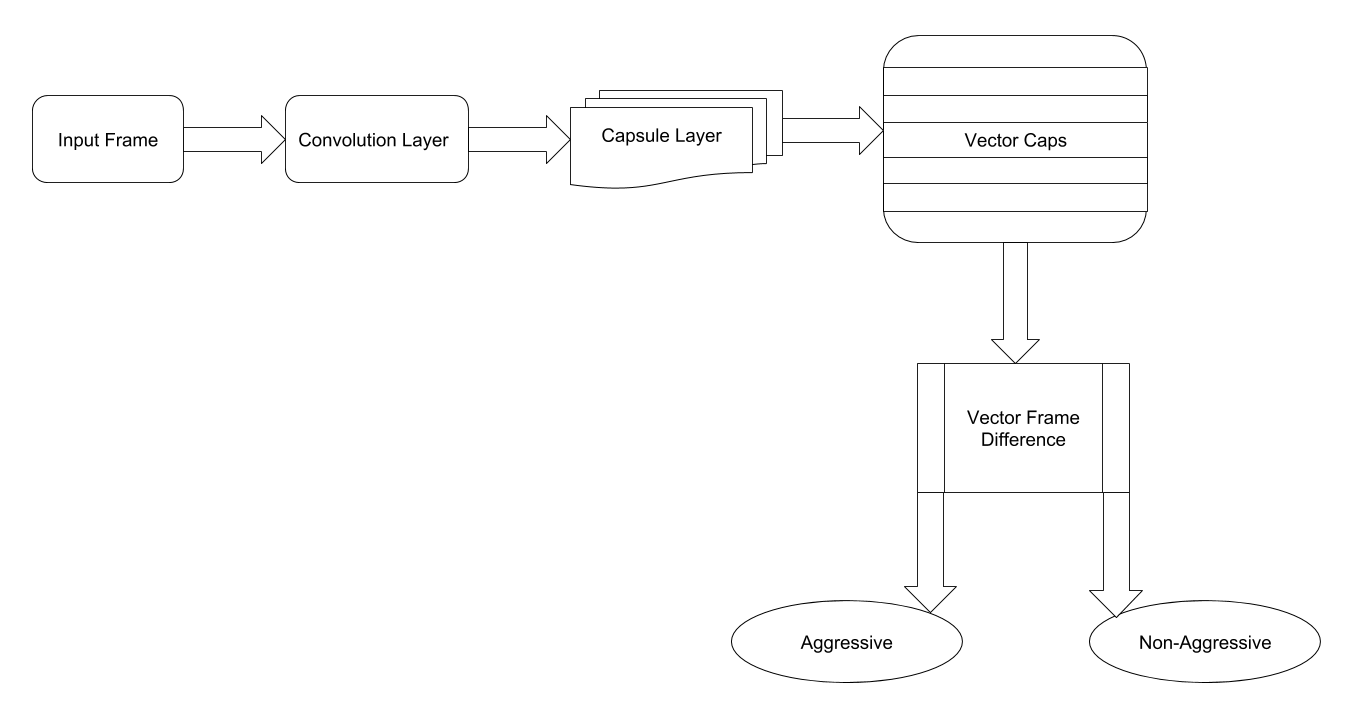
\includegraphics[width=1\textwidth]{capsframe.png}
\caption{\label{fig:framework}Proposed framework }
\end{figure}

The proposed algorithm is shown in figure 1. The algorithm starts with the primary convo-lutional layer of the capsule network algorithm showed by Geoffrey Hinton \cite{sabour2017dynamic}. This Convolutional layer
converts pixel congestions to the activity of local feature detectors which are used as input to the
primary capsules. In Capsule layer Capsules encapsulate all important information about the state
of the feature they are detecting in vector form. These Capsules encode probability of detection of
a feature as the length of their output vector as well as the state of the detected feature is encoded
as the direction in which that vector points to. Therefore, when the detected feature moves around the image or its state somehow changes,
the probability still stays the same as length of vector does not change, but its orientation changes.
Among the nested capsule layers the length of the output vector of a capsule is assumed to
represent the probability that the entity represented by the capsule is present in the current input.
A non-linear "squashing" function used to shrunk the short vectors to almost zero length and long vectors get shrunk to a length slightly below 1. The squashing function gets applied to the vector output of each capsule. ****

The length of all activity vectors extracted from the capsule layer are stored in Vector Caps
which indicates the presence of an instance. The CapsNet will detect individual feature present
in the frame and extract activation vector. From there it is possible to obtain the specific feature
vector orientation and magnitude. If a human is moving, the feature vector will change orientation
and magnitude based on the direction of the feature (E.g. Hand, Legs) moving and scaling factor
of the image from frame to frame (E.g. Human coming toward the lens would make the scaling
factor > 1 and moving away from the lens will make the scaling factor < 1). These will be
calculated for every frame. Then the vector frame difference will be calculated by dividing the
orientation distance with time taken for changing orientation. Later a SVM will classify the frame
whether it carries aggressive motion or not by comparing the threshold value and Vector Frame
Difference (VFD) value. If VFD value is less than the threshold value the frame will be considered
as Aggressive. The threshold value will be calculated through testing the average velocity and
normal velocity of human movement in any scene. The algorithm we proposing for Vector Frame
Difference is: 

For every\_feature in frame2:

	vectorframe1 = frame1.feature(CapsNet cap[featurehand])
    
	vectorframe2 = frame2.feature(CapsNet cap[featurehand])
    $$\Delta\vartheta = \frac{vectorframe2.orientation - vectorframe1.orientation}{\Delta T}$$

	

if( $\Delta \vartheta$ > threshold)
	 \{
		
        aggressive.trainSVM(vectorframe1,vectorframe2);
     \}

else	
    \{
    
    	nonaggressive.trainSVM(vectorframe1,vectorframe2);
        \}







\section{Conclusion}
Violent behavior detection can help to ensure safety of people and help law enforcement agencies to identify the perpetrator. This review task highlights the importance of the impact of detecting violence and aggressive behavior. In detecting violent scenes and to segment them, methods have to have robust spatiotemporal feature extraction and augmentation technique, focus on  hierarchical relations and ability to discriminate inherent ambiguous human actions. Current methods which tackle this interesting problem were thoroughly analyzed to shed light on the weaknesses and strengths. From this review it is apparent that there is trend of using Convolutional Neural Networks as it provides discriminative power. But CNNs are not without fault as they heavily rely on different pooling strategies resulting in information loss. CNNs also lack the ability to encode motion features inherently and have to depend on specialised motion feature mapping networks. Moreover they do not perform well in scenarios with overlapping subjects. CapsNet though also lacking the motion features, have the ability of hierarchical segmentation and input reconstruction as well as performs better on overlapping scenarios with multitude of orientational variations. After analyzing existing frameworks, this paper presents a modified and updated framework for segmentation and action recognition which are expected to handle robustness indicated in observations. Judging from the previous research in computer vision field, it is certain that it will continue to be among the best research field in the future.

\bibliographystyle{plain}
\bibliography{references}
\end{document}
